% Options for packages loaded elsewhere
\PassOptionsToPackage{unicode}{hyperref}
\PassOptionsToPackage{hyphens}{url}
%
\documentclass[
]{book}
\usepackage{lmodern}
\usepackage{amssymb,amsmath}
\usepackage{ifxetex,ifluatex}
\ifnum 0\ifxetex 1\fi\ifluatex 1\fi=0 % if pdftex
  \usepackage[T1]{fontenc}
  \usepackage[utf8]{inputenc}
  \usepackage{textcomp} % provide euro and other symbols
\else % if luatex or xetex
  \usepackage{unicode-math}
  \defaultfontfeatures{Scale=MatchLowercase}
  \defaultfontfeatures[\rmfamily]{Ligatures=TeX,Scale=1}
\fi
% Use upquote if available, for straight quotes in verbatim environments
\IfFileExists{upquote.sty}{\usepackage{upquote}}{}
\IfFileExists{microtype.sty}{% use microtype if available
  \usepackage[]{microtype}
  \UseMicrotypeSet[protrusion]{basicmath} % disable protrusion for tt fonts
}{}
\makeatletter
\@ifundefined{KOMAClassName}{% if non-KOMA class
  \IfFileExists{parskip.sty}{%
    \usepackage{parskip}
  }{% else
    \setlength{\parindent}{0pt}
    \setlength{\parskip}{6pt plus 2pt minus 1pt}}
}{% if KOMA class
  \KOMAoptions{parskip=half}}
\makeatother
\usepackage{xcolor}
\IfFileExists{xurl.sty}{\usepackage{xurl}}{} % add URL line breaks if available
\IfFileExists{bookmark.sty}{\usepackage{bookmark}}{\usepackage{hyperref}}
\hypersetup{
  pdftitle={Dasar Pemrograman R},
  pdfauthor={dimas},
  hidelinks,
  pdfcreator={LaTeX via pandoc}}
\urlstyle{same} % disable monospaced font for URLs
\usepackage{color}
\usepackage{fancyvrb}
\newcommand{\VerbBar}{|}
\newcommand{\VERB}{\Verb[commandchars=\\\{\}]}
\DefineVerbatimEnvironment{Highlighting}{Verbatim}{commandchars=\\\{\}}
% Add ',fontsize=\small' for more characters per line
\usepackage{framed}
\definecolor{shadecolor}{RGB}{248,248,248}
\newenvironment{Shaded}{\begin{snugshade}}{\end{snugshade}}
\newcommand{\AlertTok}[1]{\textcolor[rgb]{0.94,0.16,0.16}{#1}}
\newcommand{\AnnotationTok}[1]{\textcolor[rgb]{0.56,0.35,0.01}{\textbf{\textit{#1}}}}
\newcommand{\AttributeTok}[1]{\textcolor[rgb]{0.77,0.63,0.00}{#1}}
\newcommand{\BaseNTok}[1]{\textcolor[rgb]{0.00,0.00,0.81}{#1}}
\newcommand{\BuiltInTok}[1]{#1}
\newcommand{\CharTok}[1]{\textcolor[rgb]{0.31,0.60,0.02}{#1}}
\newcommand{\CommentTok}[1]{\textcolor[rgb]{0.56,0.35,0.01}{\textit{#1}}}
\newcommand{\CommentVarTok}[1]{\textcolor[rgb]{0.56,0.35,0.01}{\textbf{\textit{#1}}}}
\newcommand{\ConstantTok}[1]{\textcolor[rgb]{0.00,0.00,0.00}{#1}}
\newcommand{\ControlFlowTok}[1]{\textcolor[rgb]{0.13,0.29,0.53}{\textbf{#1}}}
\newcommand{\DataTypeTok}[1]{\textcolor[rgb]{0.13,0.29,0.53}{#1}}
\newcommand{\DecValTok}[1]{\textcolor[rgb]{0.00,0.00,0.81}{#1}}
\newcommand{\DocumentationTok}[1]{\textcolor[rgb]{0.56,0.35,0.01}{\textbf{\textit{#1}}}}
\newcommand{\ErrorTok}[1]{\textcolor[rgb]{0.64,0.00,0.00}{\textbf{#1}}}
\newcommand{\ExtensionTok}[1]{#1}
\newcommand{\FloatTok}[1]{\textcolor[rgb]{0.00,0.00,0.81}{#1}}
\newcommand{\FunctionTok}[1]{\textcolor[rgb]{0.00,0.00,0.00}{#1}}
\newcommand{\ImportTok}[1]{#1}
\newcommand{\InformationTok}[1]{\textcolor[rgb]{0.56,0.35,0.01}{\textbf{\textit{#1}}}}
\newcommand{\KeywordTok}[1]{\textcolor[rgb]{0.13,0.29,0.53}{\textbf{#1}}}
\newcommand{\NormalTok}[1]{#1}
\newcommand{\OperatorTok}[1]{\textcolor[rgb]{0.81,0.36,0.00}{\textbf{#1}}}
\newcommand{\OtherTok}[1]{\textcolor[rgb]{0.56,0.35,0.01}{#1}}
\newcommand{\PreprocessorTok}[1]{\textcolor[rgb]{0.56,0.35,0.01}{\textit{#1}}}
\newcommand{\RegionMarkerTok}[1]{#1}
\newcommand{\SpecialCharTok}[1]{\textcolor[rgb]{0.00,0.00,0.00}{#1}}
\newcommand{\SpecialStringTok}[1]{\textcolor[rgb]{0.31,0.60,0.02}{#1}}
\newcommand{\StringTok}[1]{\textcolor[rgb]{0.31,0.60,0.02}{#1}}
\newcommand{\VariableTok}[1]{\textcolor[rgb]{0.00,0.00,0.00}{#1}}
\newcommand{\VerbatimStringTok}[1]{\textcolor[rgb]{0.31,0.60,0.02}{#1}}
\newcommand{\WarningTok}[1]{\textcolor[rgb]{0.56,0.35,0.01}{\textbf{\textit{#1}}}}
\usepackage{longtable,booktabs}
% Correct order of tables after \paragraph or \subparagraph
\usepackage{etoolbox}
\makeatletter
\patchcmd\longtable{\par}{\if@noskipsec\mbox{}\fi\par}{}{}
\makeatother
% Allow footnotes in longtable head/foot
\IfFileExists{footnotehyper.sty}{\usepackage{footnotehyper}}{\usepackage{footnote}}
\makesavenoteenv{longtable}
\usepackage{graphicx,grffile}
\makeatletter
\def\maxwidth{\ifdim\Gin@nat@width>\linewidth\linewidth\else\Gin@nat@width\fi}
\def\maxheight{\ifdim\Gin@nat@height>\textheight\textheight\else\Gin@nat@height\fi}
\makeatother
% Scale images if necessary, so that they will not overflow the page
% margins by default, and it is still possible to overwrite the defaults
% using explicit options in \includegraphics[width, height, ...]{}
\setkeys{Gin}{width=\maxwidth,height=\maxheight,keepaspectratio}
% Set default figure placement to htbp
\makeatletter
\def\fps@figure{htbp}
\makeatother
\setlength{\emergencystretch}{3em} % prevent overfull lines
\providecommand{\tightlist}{%
  \setlength{\itemsep}{0pt}\setlength{\parskip}{0pt}}
\setcounter{secnumdepth}{5}
\usepackage{booktabs}
\usepackage{amsthm}
\makeatletter
\def\thm@space@setup{%
  \thm@preskip=8pt plus 2pt minus 4pt
  \thm@postskip=\thm@preskip
}
\makeatother
\usepackage[]{natbib}
\bibliographystyle{apalike}

\title{Dasar Pemrograman R}
\author{dimas}
\date{2021-01-02}

\begin{document}
\maketitle

{
\setcounter{tocdepth}{1}
\tableofcontents
}
Dasar - dasar Pemrograman R

\hypertarget{pengantar-r}{%
\chapter{Pengantar R}\label{pengantar-r}}

R adalah salah satu bahasa pemrograman yang khusus dirancang dalam menggunakan metode-metode statistika. Program R memberikan banyak kemudahan bagi pemula yang ingin memulai belajar pemrograman. Walaupun program R adalah open source, namun dengan library yang sangat lengkap membuat program R menjadi mampu digunakan untuk mengolah data dengan motode yang lengkap.

\hypertarget{pendefinisian-objek}{%
\section{Pendefinisian Objek}\label{pendefinisian-objek}}

Objek merupakan sebuah wadah untuk menyimpan informasi yang telah didefinisikan oleh pengguna R. Penyimpanan informasi ke dalam sebuah objek memberikan kemudahan bagi pengguna R untuk memanggil informasi yang sama berulang kali hanya dengan memanggil objeknya saja. Seringkali sebuah informasi memiliki banyak komponen, sehingga jika harus memanggilnya berulang kali akan menjadi sangat tidak efektif. Sehingga dengan mendefinisikannya ke dalam sebuah objek akan mempercepat proses pengerjaannya.

Terdapat beberapa cara dalam mendefinisikan objek pada R seperti yang tersajikan pada tabel berikut:

\begin{table}

\caption{\label{tab:unnamed-chunk-1}Operator Pendefinisian Objek pada R}
\centering
\begin{tabular}[t]{ll}
\toprule
Operator & Operasi\\
\midrule
<-, <<-, = & Mendefinisikan objek sebelah kiri\\
->, ->> & Mendefinisikan objek sebelah kanan\\
\bottomrule
\end{tabular}
\end{table}

Contoh penggunaannya adalah sebagai berikut:

\begin{Shaded}
\begin{Highlighting}[]
\NormalTok{x <-}\StringTok{ }\DecValTok{4}
\NormalTok{y <-}\StringTok{ }\KeywordTok{c}\NormalTok{(}\DecValTok{1}\NormalTok{, }\DecValTok{4}\NormalTok{, }\DecValTok{6}\NormalTok{, }\DecValTok{8}\NormalTok{, }\DecValTok{5}\NormalTok{)}
\NormalTok{z <-}\StringTok{ }\KeywordTok{c}\NormalTok{(}\StringTok{"Indonesia"}\NormalTok{, }\StringTok{"Raya"}\NormalTok{)}
\end{Highlighting}
\end{Shaded}

\begin{Shaded}
\begin{Highlighting}[]
\NormalTok{x}
\end{Highlighting}
\end{Shaded}

\begin{verbatim}
## [1] 4
\end{verbatim}

\begin{Shaded}
\begin{Highlighting}[]
\NormalTok{y}
\end{Highlighting}
\end{Shaded}

\begin{verbatim}
## [1] 1 4 6 8 5
\end{verbatim}

\begin{Shaded}
\begin{Highlighting}[]
\NormalTok{z}
\end{Highlighting}
\end{Shaded}

\begin{verbatim}
## [1] "Indonesia" "Raya"
\end{verbatim}

\hypertarget{paket-package}{%
\section{Paket (Package)}\label{paket-package}}

\hypertarget{datatype}{%
\chapter{Tipe Data}\label{datatype}}

Terdapat 5 tipe data pada bahasa pemrograman R. Setiap tipe data tersebut memiliki karakteristik sendiri sehingga tidak terjadi tumpang tindih dalam melakukan berbagai macam pengoperasiannya. Berikut adalah 6 tipe data pada bahasa pemrograman R:

\hypertarget{numeric}{%
\section{Numerik (Numeric)}\label{numeric}}

Tipe data numerik adalah tipe data yang berupa nilai/angka desimal. Tipe data ini merupakan tipe data yang dapat digunakan untuk melakukan operasi-operasi aritmatika seperti penjumlahan, pengurangan, perkailan, dsb. Jika kita definisikan objek \texttt{x} dengan suatu nilai/angka, maka tipe objek tersbut adalah \texttt{numeric}.

\begin{Shaded}
\begin{Highlighting}[]
\NormalTok{x <-}\StringTok{ }\FloatTok{2.6}
\KeywordTok{class}\NormalTok{(x)}
\end{Highlighting}
\end{Shaded}

\begin{verbatim}
## [1] "numeric"
\end{verbatim}

Bahkan R akan mendefinisikan objek dengan tipe \texttt{numeric} jika berikan angka tanpa desimal.

\begin{Shaded}
\begin{Highlighting}[]
\NormalTok{x <-}\StringTok{ }\DecValTok{5}
\KeywordTok{class}\NormalTok{(x)}
\end{Highlighting}
\end{Shaded}

\begin{verbatim}
## [1] "numeric"
\end{verbatim}

\hypertarget{integer}{%
\section{Bilangan Bulat (Integer)}\label{integer}}

Seperti yang kita tahu bahwa pendefinisian angka pada suatu objek akan secara otomatis membuat objek tersebut bertipe \texttt{numeric}. Sedangkan untuk mendefinisikan objek dengan tipe \texttt{integer} harus mendefinisikan secara khusus objek tersebut dengan perintah \texttt{as.integer}.

\begin{Shaded}
\begin{Highlighting}[]
\NormalTok{x <-}\StringTok{ }\KeywordTok{as.integer}\NormalTok{(}\DecValTok{5}\NormalTok{)}
\KeywordTok{class}\NormalTok{(x)}
\end{Highlighting}
\end{Shaded}

\begin{verbatim}
## [1] "integer"
\end{verbatim}

Selain itu kita dapat mendefinisikan sebuah objek yang bertipe \texttt{integer} dengan menambahkan huruf \texttt{L} kapital pada akhir angka.

\begin{Shaded}
\begin{Highlighting}[]
\NormalTok{x <-}\StringTok{ }\NormalTok{3L}
\KeywordTok{class}\NormalTok{(x)}
\end{Highlighting}
\end{Shaded}

\begin{verbatim}
## [1] "integer"
\end{verbatim}

Bagaimana jika kita berikan angka desimal pada objek yang kita definisikan sebagai \texttt{integer}?

\begin{Shaded}
\begin{Highlighting}[]
\NormalTok{x <-}\StringTok{ }\KeywordTok{as.integer}\NormalTok{(}\FloatTok{3.76}\NormalTok{)}
\end{Highlighting}
\end{Shaded}

\hypertarget{complex}{%
\section{Bilangan Kompleks (Complex)}\label{complex}}

Bilangan kompleks dalam matematika adalah bilangan yang didefinisikan dengan \(a + bi\), dengan \(a\) dan \(b\) adalah bilangan real. Sedangkan \(i\) adalah bilangan imajiner dan menyebabkan \(bi\) menjadi imajiner. Bilangan imajiner sendiri memiliki sifat \(i^{2}=1\). Kita harus secara langsung mendefinisikan objek sebagai bilangan kompleks agar mendapatkan sebuah objek yang bertipe \texttt{complex}.

\begin{Shaded}
\begin{Highlighting}[]
\NormalTok{x <-}\StringTok{ }\DecValTok{2} \OperatorTok{+}\StringTok{ }\NormalTok{4i}
\KeywordTok{class}\NormalTok{(x)}
\end{Highlighting}
\end{Shaded}

\begin{verbatim}
## [1] "complex"
\end{verbatim}

\hypertarget{logical}{%
\section{Logika (Logical)}\label{logical}}

Objek dengan tipe logika adalah objek yang hanya memiliki 2 nilai saja yaitu \texttt{TRUE} dan \texttt{FALSE}.

\begin{Shaded}
\begin{Highlighting}[]
\NormalTok{x <-}\StringTok{ }\OtherTok{TRUE}
\KeywordTok{class}\NormalTok{(x)}
\end{Highlighting}
\end{Shaded}

\begin{verbatim}
## [1] "logical"
\end{verbatim}

\hypertarget{character}{%
\section{Teks (Character)}\label{character}}

Pendefinisian objek dengan tipe teks (\texttt{character}) merupakan hal yang cukup mudah. Kita perlu menambahkan tanda petik \texttt{"} pada awal dan akhir teks. Setelah itu objek akan terdefinisikan sebagai \texttt{character}.

\begin{Shaded}
\begin{Highlighting}[]
\NormalTok{x <-}\StringTok{ "Aplikasi Komputer"}
\KeywordTok{class}\NormalTok{(x)}
\end{Highlighting}
\end{Shaded}

\begin{verbatim}
## [1] "character"
\end{verbatim}

\begin{Shaded}
\begin{Highlighting}[]
\NormalTok{x}
\end{Highlighting}
\end{Shaded}

\begin{verbatim}
## [1] "Aplikasi Komputer"
\end{verbatim}

Apakah tipe data dari objek yang didefinisikan dengan nilai \texttt{"2.4"}?

\hypertarget{factor}{%
\section{Faktor (Factor)}\label{factor}}

Faktor adalah tipe data pada bahasa pemrograman R yang digunakan untuk mendefinisikan sebuah objek menjadi sebuah objek dengan tipe data kategorik. Perintah yang digunakan untuk merubah sebuah objek menjadi sebuah faktor adalah \texttt{factor()}.

\begin{Shaded}
\begin{Highlighting}[]
\NormalTok{x <-}\StringTok{ }\KeywordTok{factor}\NormalTok{(}\KeywordTok{c}\NormalTok{(}\DecValTok{1}\NormalTok{, }\DecValTok{2}\NormalTok{, }\DecValTok{3}\NormalTok{))}
\NormalTok{y <-}\StringTok{ }\KeywordTok{factor}\NormalTok{(}\KeywordTok{c}\NormalTok{(}\StringTok{"SD"}\NormalTok{, }\StringTok{"SMP"}\NormalTok{, }\StringTok{"SMA"}\NormalTok{, }\StringTok{"SMA"}\NormalTok{, }\StringTok{"PT"}\NormalTok{))}
\NormalTok{x}
\end{Highlighting}
\end{Shaded}

\begin{verbatim}
## [1] 1 2 3
## Levels: 1 2 3
\end{verbatim}

\begin{Shaded}
\begin{Highlighting}[]
\NormalTok{y}
\end{Highlighting}
\end{Shaded}

\begin{verbatim}
## [1] SD  SMP SMA SMA PT 
## Levels: PT SD SMA SMP
\end{verbatim}

Sebuah objek yang telah didefinisikan sebagaik faktor akan memiliki \texttt{levels} yang merupakan daftar kategori yang terdapat pada objek tersebut. Kita dapat menggunakan perintah \texttt{levels} untuk dapat memunculkan \texttt{levels} nya saja.

\begin{Shaded}
\begin{Highlighting}[]
\KeywordTok{levels}\NormalTok{(x)}
\end{Highlighting}
\end{Shaded}

\begin{verbatim}
## [1] "1" "2" "3"
\end{verbatim}

\begin{Shaded}
\begin{Highlighting}[]
\KeywordTok{levels}\NormalTok{(y)}
\end{Highlighting}
\end{Shaded}

\begin{verbatim}
## [1] "PT"  "SD"  "SMA" "SMP"
\end{verbatim}

\begin{itemize}
\tightlist
\item
  Apa perbedaan \emph{output} dari objek yang bertipe \texttt{factor} dengan objek yang bertipe \texttt{numeric}?
\item
  Apa perbedaan \emph{output} dari objek yang bertipe \texttt{factor} dengan objek yang bertipe \texttt{character}?
\end{itemize}

\hypertarget{struktur-data}{%
\chapter{Struktur Data}\label{struktur-data}}

Struktur data pada bahasa pemrograman R adalah sebuah konsep yang digunakan untuk menyimpan data berdasarkan kebutuhannya. Berdasarkan struktur datanya, terdapat 4 struktur data yang dapat kita definisikan pada program R:

\begin{itemize}
\tightlist
\item
  Vektor (\texttt{vector})
\item
  Matriks (\texttt{matrix})
\item
  Pendafaran (\texttt{list})
\item
  Kerangka Data (\texttt{data.frame})
\end{itemize}

\hypertarget{vector}{%
\section{Vektor (Vector)}\label{vector}}

Vektor adalah struktur data yang paling sederhana pada bahasa pemrograman R. Vektor memuat barisan data dengan tipe data yang sama. Pendefinisian vektor dilakukan dengan menggunakan perintah \texttt{c()}. Semua data ditulis didalam tanda kurung dan setiap data dipisahkan dengan tanda koma \texttt{,}.

\begin{Shaded}
\begin{Highlighting}[]
\NormalTok{x <-}\StringTok{ }\KeywordTok{c}\NormalTok{(}\DecValTok{1}\OperatorTok{:}\DecValTok{5}\NormalTok{)}
\NormalTok{x}
\end{Highlighting}
\end{Shaded}

\begin{verbatim}
## [1] 1 2 3 4 5
\end{verbatim}

\begin{Shaded}
\begin{Highlighting}[]
\NormalTok{y <-}\StringTok{ }\KeywordTok{c}\NormalTok{(}\StringTok{"Hipertensi"}\NormalTok{, }\StringTok{"Diabetes"}\NormalTok{, }\StringTok{"Asam Urat"}\NormalTok{)}
\NormalTok{y}
\end{Highlighting}
\end{Shaded}

\begin{verbatim}
## [1] "Hipertensi" "Diabetes"   "Asam Urat"
\end{verbatim}

\begin{Shaded}
\begin{Highlighting}[]
\KeywordTok{length}\NormalTok{(x)}
\end{Highlighting}
\end{Shaded}

\begin{verbatim}
## [1] 5
\end{verbatim}

\begin{Shaded}
\begin{Highlighting}[]
\KeywordTok{length}\NormalTok{(y)}
\end{Highlighting}
\end{Shaded}

\begin{verbatim}
## [1] 3
\end{verbatim}

Apa yang terjadi apabila sebuah vektor diisi dengan 2 tipe data? misalnya \texttt{c(12,\ 4,\ TRUE)}

Selanjutnya kita dapat memanggil anggota dari sebuah objek \texttt{vector} dengan menggunakan tanda \texttt{{[}x{]}} setelah objek dengan \texttt{x} adalah nilai yang menyatakan \emph{data ke-x}.

\begin{Shaded}
\begin{Highlighting}[]
\NormalTok{x[}\DecValTok{2}\NormalTok{]}
\end{Highlighting}
\end{Shaded}

\begin{verbatim}
## [1] 2
\end{verbatim}

\begin{Shaded}
\begin{Highlighting}[]
\NormalTok{y[}\DecValTok{3}\NormalTok{]}
\end{Highlighting}
\end{Shaded}

\begin{verbatim}
## [1] "Asam Urat"
\end{verbatim}

\hypertarget{matrix}{%
\section{Matriks (Matrix)}\label{matrix}}

Sama halnya dengan vektor, matriks merupakan struktur data yang hanya dapat menyimpan 1 tipe data saja. Perbedaan antara struktur data `matrix' dengan `vector' berada pada dimensi datanya. Vektor merupakan struktur data berdimensi 1 (hanya memiliki panjang data). Sedangkan matriks adalah struktur data yang berdimensi 2 (memiliki dimensi dan panjang data).

Pendefinisian matriks dilakukan dengan menggunakan perintah \texttt{matrix} dengan \texttt{syntax}: \texttt{matrix(data,\ nrow,\ ncol,\ byrow=FALSE)}.

\begin{Shaded}
\begin{Highlighting}[]
\NormalTok{x <-}\StringTok{ }\KeywordTok{matrix}\NormalTok{(}
  \KeywordTok{c}\NormalTok{(}\DecValTok{1}\OperatorTok{:}\DecValTok{8}\NormalTok{), }\DecValTok{2}\NormalTok{, }\DecValTok{4}
\NormalTok{)}
\NormalTok{x}
\end{Highlighting}
\end{Shaded}

\begin{verbatim}
##      [,1] [,2] [,3] [,4]
## [1,]    1    3    5    7
## [2,]    2    4    6    8
\end{verbatim}

\begin{Shaded}
\begin{Highlighting}[]
\KeywordTok{dim}\NormalTok{(x)}
\end{Highlighting}
\end{Shaded}

\begin{verbatim}
## [1] 2 4
\end{verbatim}

dengan:

\begin{itemize}
\tightlist
\item
  \texttt{data} adalah data yang akan kita gunakan
\item
  \texttt{nrow} adalah jumlah baris
\item
  \texttt{ncol} adalah jumlah kolom
\item
  \texttt{byrow} adalah perintah opsional untuk memilih agar data yang kita miliki didaftarkan berdasarkan baris atau kolom
\end{itemize}

Apakah yang akan terjadi apabila kita menggunakan \texttt{byrow=FALSE} dan \texttt{byrow=TRUE}?

Berbeda dengan objek yang berupa \texttt{vector}, pemanggilan data pada objek \texttt{matrix} menggunakan tanda \texttt{{[}x,y{]}} dimana \texttt{x} adalah \emph{data baris ke-x} dan \texttt{y} adalah \emph{data kolom ke-y}. Apabila kita menggunakan tanda \texttt{{[}x,{]}} saja, maka kita memanggil semua data pada \emph{baris ke-x}. Sedangkan apabila kita menggunakan tanda \texttt{{[},y{]}} saja, maka kita memanggil semua data pada \emph{kolom ke-y}.

\begin{Shaded}
\begin{Highlighting}[]
\NormalTok{x[}\DecValTok{2}\NormalTok{,}\DecValTok{3}\NormalTok{]}
\end{Highlighting}
\end{Shaded}

\begin{verbatim}
## [1] 6
\end{verbatim}

\begin{Shaded}
\begin{Highlighting}[]
\NormalTok{x[}\DecValTok{2}\NormalTok{,]}
\end{Highlighting}
\end{Shaded}

\begin{verbatim}
## [1] 2 4 6 8
\end{verbatim}

\begin{Shaded}
\begin{Highlighting}[]
\NormalTok{x[,}\DecValTok{4}\NormalTok{]}
\end{Highlighting}
\end{Shaded}

\begin{verbatim}
## [1] 7 8
\end{verbatim}

\begin{Shaded}
\begin{Highlighting}[]
\NormalTok{x[}\DecValTok{6}\NormalTok{]}
\end{Highlighting}
\end{Shaded}

\begin{verbatim}
## [1] 6
\end{verbatim}

Catatan: \texttt{x} dan \texttt{y} pada \texttt{{[}x,y{]}} dapat berupa \texttt{vector}.

\hypertarget{list}{%
\section{Daftar (List)}\label{list}}

Struktur data \texttt{list} dalam R adalah struktur data yang dapat mendaftarkan beberapa objek sekaligus tanpa perlu khawatir dengan tipe data yang berbeda. Struktur data `list' dapat juga dikatakan sebagai vektor yang dapat menyimpan berbagai macam objek. Pendefinisian list dilakukan dengan menggunakan perintah \texttt{list()}.

\begin{Shaded}
\begin{Highlighting}[]
\NormalTok{a <-}\StringTok{ }\KeywordTok{c}\NormalTok{(}\DecValTok{1}\NormalTok{, }\DecValTok{3}\NormalTok{, }\DecValTok{6}\NormalTok{, }\DecValTok{2}\NormalTok{)}
\NormalTok{b <-}\StringTok{ }\KeywordTok{c}\NormalTok{(}\StringTok{"Apa"}\NormalTok{, }\StringTok{"kabar"}\NormalTok{, }\StringTok{"anda"}\NormalTok{, }\StringTok{"hari"}\NormalTok{, }\StringTok{"ini"}\NormalTok{, }\StringTok{"?"}\NormalTok{)}
\NormalTok{c <-}\StringTok{ }\KeywordTok{c}\NormalTok{(}\OtherTok{TRUE}\NormalTok{, }\OtherTok{FALSE}\NormalTok{, }\OtherTok{FALSE}\NormalTok{, }\OtherTok{FALSE}\NormalTok{, }\OtherTok{TRUE}\NormalTok{)}
\NormalTok{x <-}\StringTok{ }\KeywordTok{list}\NormalTok{(}\DataTypeTok{a=}\NormalTok{a, }\DataTypeTok{b=}\NormalTok{b, }\DataTypeTok{c=}\NormalTok{c)}
\NormalTok{x}
\end{Highlighting}
\end{Shaded}

\begin{verbatim}
## $a
## [1] 1 3 6 2
## 
## $b
## [1] "Apa"   "kabar" "anda"  "hari"  "ini"   "?"    
## 
## $c
## [1]  TRUE FALSE FALSE FALSE  TRUE
\end{verbatim}

Selanjutnya kita dapat memanggil masing-masing objek pada sebuah list dengan \texttt{syntax}: \texttt{ListObject\$ObjekInList} atau dengan menggunakan \texttt{{[}{[}x{]}{]}} dimana \texttt{x} adalah sebuah angka yang merujuk pada \textbf{daftar ke berapa}.

\begin{Shaded}
\begin{Highlighting}[]
\NormalTok{x}\OperatorTok{$}\NormalTok{a}
\end{Highlighting}
\end{Shaded}

\begin{verbatim}
## [1] 1 3 6 2
\end{verbatim}

\begin{Shaded}
\begin{Highlighting}[]
\NormalTok{x[[}\DecValTok{3}\NormalTok{]]}
\end{Highlighting}
\end{Shaded}

\begin{verbatim}
## [1]  TRUE FALSE FALSE FALSE  TRUE
\end{verbatim}

\hypertarget{dataframe}{%
\section{Kerangka Data (Data Frame)}\label{dataframe}}

Struktur data yang berupa \emph{data frame} (\texttt{data.frame}) merupakan struktur data yang akan paling sering kita gunakan dalam pengolahan data. Struktur data ini digunakan untuk mendefinisikan sebuah tabel data yang mana setiap kolom adalah nama-nama objek/variabel pada \emph{data frame} tersebut. Setiap objek/variabel dalam \texttt{data.frame} merupakan sebuah \texttt{vector}. Artinya setiap objek/variabel dalam \texttt{data.frame} hanya dapat memiliki 1 tipe data saja. Selain itu setiap objek/variabel yang berada dalam \texttt{data.frame} harus memiliki jumlah data (\texttt{length()}) yang sama.

Perintah \texttt{data.frame()} adalah perintah yang digunakan untuk medefinisikan sebuah objek sebagai sebuah data frame.

\begin{Shaded}
\begin{Highlighting}[]
\NormalTok{nama <-}\StringTok{ }\KeywordTok{c}\NormalTok{(}\StringTok{"Ahmad"}\NormalTok{, }\StringTok{"Ganjar"}\NormalTok{, }\StringTok{"Lusi"}\NormalTok{, }\StringTok{"Andina"}\NormalTok{, }\StringTok{"Elok"}\NormalTok{)}
\NormalTok{jk   <-}\StringTok{ }\KeywordTok{factor}\NormalTok{(}\KeywordTok{c}\NormalTok{(}\StringTok{"Laki-laki"}\NormalTok{, }\StringTok{"Laki-laki"}\NormalTok{, }\StringTok{"Perempuan"}\NormalTok{, }\StringTok{"Perempuan"}\NormalTok{, }\StringTok{"Perempuan"}\NormalTok{))}
\NormalTok{tb   <-}\StringTok{ }\KeywordTok{c}\NormalTok{(}\DecValTok{170}\NormalTok{, }\DecValTok{169}\NormalTok{, }\DecValTok{160}\NormalTok{, }\DecValTok{154}\NormalTok{, }\DecValTok{163}\NormalTok{)}
\NormalTok{bb   <-}\StringTok{ }\KeywordTok{c}\NormalTok{(}\DecValTok{70}\NormalTok{, }\DecValTok{67}\NormalTok{, }\DecValTok{45}\NormalTok{, }\DecValTok{40}\NormalTok{, }\DecValTok{52}\NormalTok{)}
\NormalTok{x    <-}\StringTok{ }\KeywordTok{data.frame}\NormalTok{(nama, jk, tb, bb)}
\NormalTok{x}
\end{Highlighting}
\end{Shaded}

\begin{verbatim}
##     nama        jk  tb bb
## 1  Ahmad Laki-laki 170 70
## 2 Ganjar Laki-laki 169 67
## 3   Lusi Perempuan 160 45
## 4 Andina Perempuan 154 40
## 5   Elok Perempuan 163 52
\end{verbatim}

\begin{table}

\caption{\label{tab:unnamed-chunk-21}Data Mahasiswa 2020}
\centering
\begin{tabular}[t]{llrr}
\toprule
nama & jk & tb & bb\\
\midrule
Ahmad & Laki-laki & 170 & 70\\
Ganjar & Laki-laki & 169 & 67\\
Lusi & Perempuan & 160 & 45\\
Andina & Perempuan & 154 & 40\\
Elok & Perempuan & 163 & 52\\
\bottomrule
\end{tabular}
\end{table}

Selanjutnya untuk memanggil objek/variabel pada sebuah \texttt{data.frame} mirip dengan memanggil data pada sebuah \texttt{matrix}. Selain itu kita dapat pula memanggil dengan cara menyebutkan nama objek/variabel pada \texttt{data.frame} tersebut.

\begin{Shaded}
\begin{Highlighting}[]
\NormalTok{x[,}\DecValTok{2}\NormalTok{]}
\end{Highlighting}
\end{Shaded}

\begin{verbatim}
## [1] Laki-laki Laki-laki Perempuan Perempuan Perempuan
## Levels: Laki-laki Perempuan
\end{verbatim}

\begin{Shaded}
\begin{Highlighting}[]
\NormalTok{x[}\DecValTok{4}\NormalTok{,]}
\end{Highlighting}
\end{Shaded}

\begin{verbatim}
##     nama        jk  tb bb
## 4 Andina Perempuan 154 40
\end{verbatim}

\begin{Shaded}
\begin{Highlighting}[]
\NormalTok{x}\OperatorTok{$}\NormalTok{nama}
\end{Highlighting}
\end{Shaded}

\begin{verbatim}
## [1] "Ahmad"  "Ganjar" "Lusi"   "Andina" "Elok"
\end{verbatim}

\begin{Shaded}
\begin{Highlighting}[]
\NormalTok{x[,}\KeywordTok{c}\NormalTok{(}\StringTok{'jk'}\NormalTok{, }\StringTok{'nama'}\NormalTok{)]}
\end{Highlighting}
\end{Shaded}

\begin{verbatim}
##          jk   nama
## 1 Laki-laki  Ahmad
## 2 Laki-laki Ganjar
## 3 Perempuan   Lusi
## 4 Perempuan Andina
## 5 Perempuan   Elok
\end{verbatim}

\hypertarget{operator---operator-pada-r}{%
\chapter{Operator - operator pada R}\label{operator---operator-pada-r}}

Operator - operator pada R adalah perintah untuk melakukan suatu operasi seperti operasi artimatika, logika dan relasi. Secara umum terdapat 4 tipe operator pada R, yaitu:

\begin{itemize}
\tightlist
\item
  Operator Aritmatika
\item
  Operator Logika
\item
  Operator Relasi
\end{itemize}

\hypertarget{operator}{%
\section{Operator Aritmatika}\label{operator}}

Operator artimatika adalah operator yang digunakan untuk melakukan komputasi dengan menggunakan operasi - operasi matematika seperti penjumlahan, pengurangan, dll. Berikut adalah daftar operator aritmatika pada R:

\begin{table}

\caption{\label{tab:unnamed-chunk-23}Operator Aritmatika pada R}
\centering
\begin{tabular}[t]{cc}
\toprule
Operator & Operasi\\
\midrule
+ & Penjumlahan\\
- & Pengurangan\\
* & Perkalian\\
/ & Pembagian\\
\textasciicircum{} & Perpangkatan\\
\addlinespace
\%\% & Modulo\\
\bottomrule
\end{tabular}
\end{table}

Operator umumnya digunakan untuk pengoperasian pada objek bertipe \texttt{numeric} atau \texttt{integer} dengan struktur data berupa \texttt{vector} dan \texttt{matrix}. Berikut adalah contoh penggunaannya:

\begin{Shaded}
\begin{Highlighting}[]
\NormalTok{x <-}\StringTok{ }\DecValTok{3}
\NormalTok{y <-}\StringTok{ }\DecValTok{5}
\end{Highlighting}
\end{Shaded}

\begin{table}

\caption{\label{tab:unnamed-chunk-25}Hasil Penggunaan Operator pada R}
\centering
\begin{tabular}[t]{ccc}
\toprule
Operator & Operasi & Hasil\\
\midrule
+ & x + y & 8.0\\
- & x - y & -2.0\\
* & x * y & 15.0\\
/ & x / y & 0.6\\
\textasciicircum{} & x \textasciicircum{} y & 243.0\\
\addlinespace
\%\% & x \%\% y & 3.0\\
\bottomrule
\end{tabular}
\end{table}

\hypertarget{operator-logika}{%
\section{Operator Logika}\label{operator-logika}}

Operator logika akan menghasilkan nilai \texttt{TRUE} dan \texttt{FALSE}. Seperti halnya logika matematika, terdapat 2 operator logika yaitu \emph{dan} (\texttt{AND}), \emph{atau} (\texttt{OR}) dan ingkaran (\texttt{NOT}). Berikut adalah daftar operator logika pada R:

\begin{table}

\caption{\label{tab:unnamed-chunk-26}Operator Logika pada R}
\centering
\begin{tabular}[t]{cc}
\toprule
Operator & Operasi\\
\midrule
! & Bukan/Ingkaran\\
\& & Logika DAN pada masing-masing anggota objek\\
\&\& & Logika DAN\\
| & Logika ATAU\\
|| & Logika ATAU pada masing-masing anggota objek\\
\bottomrule
\end{tabular}
\end{table}

Berikut adalah contoh hasil penggunaannya:

\begin{Shaded}
\begin{Highlighting}[]
\NormalTok{x <-}\StringTok{ }\KeywordTok{c}\NormalTok{(}\OtherTok{TRUE}\NormalTok{, }\OtherTok{FALSE}\NormalTok{, }\DecValTok{5}\NormalTok{)}
\NormalTok{y <-}\StringTok{ }\KeywordTok{c}\NormalTok{(}\OtherTok{TRUE}\NormalTok{, }\OtherTok{FALSE}\NormalTok{, }\OtherTok{FALSE}\NormalTok{)}
\NormalTok{z <-}\StringTok{ }\KeywordTok{c}\NormalTok{(}\OtherTok{FALSE}\NormalTok{, }\OtherTok{TRUE}\NormalTok{, }\OtherTok{TRUE}\NormalTok{)}

\OperatorTok{!}\NormalTok{x}
\end{Highlighting}
\end{Shaded}

\begin{verbatim}
## [1] FALSE  TRUE FALSE
\end{verbatim}

\begin{Shaded}
\begin{Highlighting}[]
\NormalTok{x}\OperatorTok{&}\NormalTok{y}
\end{Highlighting}
\end{Shaded}

\begin{verbatim}
## [1]  TRUE FALSE FALSE
\end{verbatim}

\begin{Shaded}
\begin{Highlighting}[]
\NormalTok{x}\OperatorTok{&&}\NormalTok{z}
\end{Highlighting}
\end{Shaded}

\begin{verbatim}
## [1] FALSE
\end{verbatim}

\begin{Shaded}
\begin{Highlighting}[]
\NormalTok{x}\OperatorTok{|}\NormalTok{y}
\end{Highlighting}
\end{Shaded}

\begin{verbatim}
## [1]  TRUE FALSE  TRUE
\end{verbatim}

\begin{Shaded}
\begin{Highlighting}[]
\NormalTok{x}\OperatorTok{||}\NormalTok{z}
\end{Highlighting}
\end{Shaded}

\begin{verbatim}
## [1] TRUE
\end{verbatim}

\begin{table}

\caption{\label{tab:unnamed-chunk-28}Hasil Penggunaan Operator Logika}
\centering
\begin{tabular}[t]{llllll}
\toprule
P1 & P2 & NegasiP1 & NegasiP2 & DAN & ATAU\\
\midrule
TRUE & TRUE & FALSE & FALSE & TRUE & TRUE\\
TRUE & FALSE & FALSE & TRUE & FALSE & TRUE\\
FALSE & TRUE & TRUE & FALSE & FALSE & TRUE\\
FALSE & FALSE & TRUE & TRUE & FALSE & FALSE\\
\bottomrule
\end{tabular}
\end{table}

\hypertarget{relational}{%
\section{Operator Relasi}\label{relational}}

Operator relasi adalah operator yang digunakan untuk membandingkan 2 buah nilai/objek. Hasil \emph{output} dari operator relasi ini adalah \texttt{TRUE} dan \texttt{FALSE}. Berikut adalah daftar operator relasi:

\begin{table}

\caption{\label{tab:unnamed-chunk-29}Operasi Relasi pada R}
\centering
\begin{tabular}[t]{ll}
\toprule
Operator & Operasi\\
\midrule
< & Kurang dari\\
<= & Kurang dari sama dengan\\
> & Lebih dari\\
>= & Lebih dari sama dengan\\
== & Sama dengan\\
\addlinespace
!= & Tidak sama dengan\\
\bottomrule
\end{tabular}
\end{table}

Operator relasi dapat dioperasikan layaknya operator logika. Berikut adalah contoh penggunaannya:

\begin{Shaded}
\begin{Highlighting}[]
\NormalTok{x <-}\StringTok{ }\DecValTok{3}
\NormalTok{y <-}\StringTok{ }\DecValTok{7}
\NormalTok{z <-}\StringTok{ }\DecValTok{7}
\NormalTok{x}\OperatorTok{<}\NormalTok{y}
\end{Highlighting}
\end{Shaded}

\begin{verbatim}
## [1] TRUE
\end{verbatim}

\begin{Shaded}
\begin{Highlighting}[]
\NormalTok{x}\OperatorTok{>}\NormalTok{y}
\end{Highlighting}
\end{Shaded}

\begin{verbatim}
## [1] FALSE
\end{verbatim}

\begin{Shaded}
\begin{Highlighting}[]
\NormalTok{x}\OperatorTok{<=}\NormalTok{y}
\end{Highlighting}
\end{Shaded}

\begin{verbatim}
## [1] TRUE
\end{verbatim}

\begin{Shaded}
\begin{Highlighting}[]
\NormalTok{y}\OperatorTok{<=}\NormalTok{z}
\end{Highlighting}
\end{Shaded}

\begin{verbatim}
## [1] TRUE
\end{verbatim}

\begin{Shaded}
\begin{Highlighting}[]
\NormalTok{x}\OperatorTok{!=}\NormalTok{y}
\end{Highlighting}
\end{Shaded}

\begin{verbatim}
## [1] TRUE
\end{verbatim}

\begin{Shaded}
\begin{Highlighting}[]
\NormalTok{y}\OperatorTok{==}\NormalTok{z}
\end{Highlighting}
\end{Shaded}

\begin{verbatim}
## [1] TRUE
\end{verbatim}

\hypertarget{plot-dengan-ggplot2}{%
\chapter{\texorpdfstring{Plot dengan \texttt{ggplot2}}{Plot dengan ggplot2}}\label{plot-dengan-ggplot2}}

Plot adalah salah satu hal mendasar yang dapat digunakan untuk menggambarkan distribusi data. Program R pun memiliki perintah - perintah untuk membuat sebuah plot. Namun perintah - perintah tersebut masih merupakan perintah yang sederhana. Hasilnya, gambar kurang menarik untuk disajikan pada khalayak umum.

\texttt{ggplot2} merupakan sebuah paket yang dapat digunakan pada program R dengan cara melakukan instalasi terlebih dahulu menggunakan perintah \texttt{install.package("ggplot2")}. Paket \texttt{ggplot2} memberikan fasilitas bagi penggunanya dalam membuat sebuah plot yang menarik untuk dilihat. Setelah anda memahami jenis-jenis plot beserta cara penggunaannya, kita dapat menggunakan paket \texttt{ggpubr} yang telah disusun khusus untuk kebutuhan publikasi/penerbitan.

Setelah instalasi paket \texttt{ggplot2} selesai, selanjutnya kita dapat memanggil paket tersebut dengan perintah

\begin{Shaded}
\begin{Highlighting}[]
\KeywordTok{library}\NormalTok{(ggplot2)}
\end{Highlighting}
\end{Shaded}

\hypertarget{bar-plot}{%
\section{Bar Plot}\label{bar-plot}}

Grafik batang merupakan grafik yang digunakan untuk menunjukkan frekuensi dari dara. Grafik batang lebih sering digunakan untuk menunjukkan perbedaan jumlah dari data yang bertipe kategorik seperti jenis kelamin, asal daerah, status perniahan, dsb. Selanjutnya kita akan membuat sebuah grafik batang dengan menggunakan data berikut:

\begin{Shaded}
\begin{Highlighting}[]
\NormalTok{jpc <-}\StringTok{ }\KeywordTok{c}\NormalTok{(}\DecValTok{34}\NormalTok{, }\DecValTok{25}\NormalTok{, }\DecValTok{69}\NormalTok{, }\DecValTok{40}\NormalTok{, }\DecValTok{30}\NormalTok{, }\DecValTok{32}\NormalTok{, }\DecValTok{45}\NormalTok{)}
\NormalTok{hr  <-}\StringTok{ }\KeywordTok{c}\NormalTok{(}\StringTok{"Sen"}\NormalTok{, }\StringTok{"Sel"}\NormalTok{, }\StringTok{"Rab"}\NormalTok{, }\StringTok{"Kam"}\NormalTok{, }\StringTok{"Jum"}\NormalTok{, }\StringTok{"Sab"}\NormalTok{, }\StringTok{"Min"}\NormalTok{)}
\NormalTok{x   <-}\StringTok{ }\KeywordTok{data.frame}\NormalTok{(}\DataTypeTok{Hari =}\NormalTok{ hr, }\DataTypeTok{Pasien =}\NormalTok{ jpc)}
\NormalTok{x}
\end{Highlighting}
\end{Shaded}

\begin{verbatim}
##   Hari Pasien
## 1  Sen     34
## 2  Sel     25
## 3  Rab     69
## 4  Kam     40
## 5  Jum     30
## 6  Sab     32
## 7  Min     45
\end{verbatim}

Terdapat perintah \texttt{barplot} dalam \texttt{R} yang merupakan perintah yang sudah tersedia saat melakukan instalasi \texttt{R}. Walapun perintah \texttt{barplot} dapat kita gunakan, namun hasil yang diberikan sangat sederhana dan lebih cocok digunakan untuk sebuah laporan. Berikut adalah cara menggunakan perintah \texttt{barplot}:

\begin{Shaded}
\begin{Highlighting}[]
\KeywordTok{barplot}\NormalTok{(x}\OperatorTok{$}\NormalTok{Pasien, }
        \DataTypeTok{names.arg =}\NormalTok{ x}\OperatorTok{$}\NormalTok{Hari)}
\end{Highlighting}
\end{Shaded}

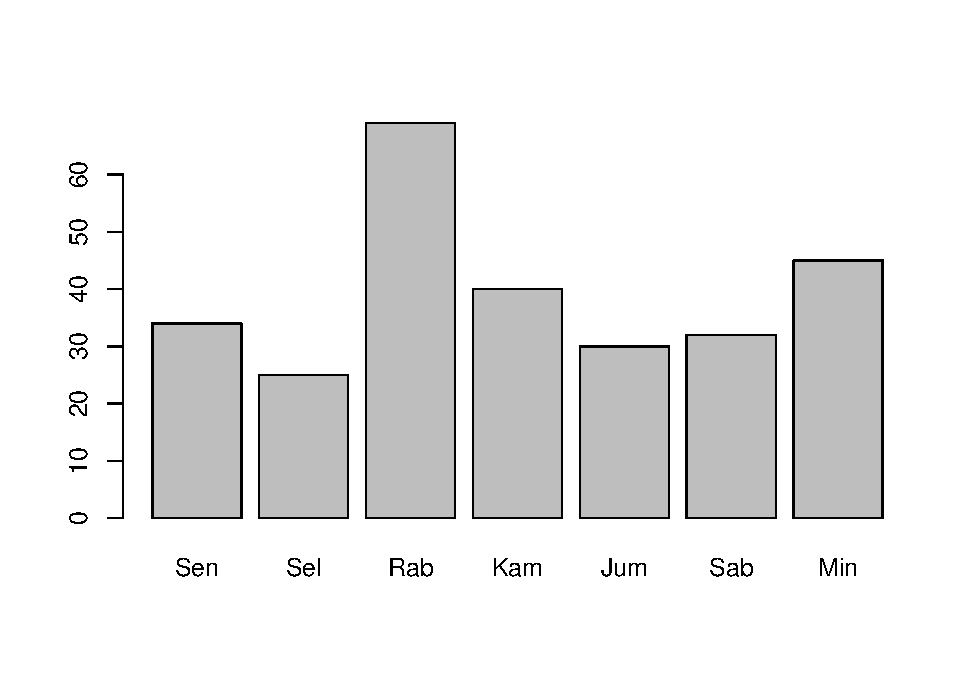
\includegraphics{dr_files/figure-latex/unnamed-chunk-33-1.pdf}

Selanjutnya kita akan menggunakan paket \texttt{ggplot2} untuk menyajikan grafik batang yang lebih menarik. Berikut adalah perintah untuk membuat grafik batang dengan menggunakan paket \texttt{ggplot2}:

\begin{Shaded}
\begin{Highlighting}[]
\NormalTok{p <-}\StringTok{ }\KeywordTok{ggplot}\NormalTok{(x, }\KeywordTok{aes}\NormalTok{(Hari)) }\OperatorTok{+}\StringTok{ }
\StringTok{  }\KeywordTok{geom_bar}\NormalTok{(}\KeywordTok{aes}\NormalTok{(}\DataTypeTok{weight=}\NormalTok{Pasien, }\DataTypeTok{fill=}\NormalTok{Hari, }\DataTypeTok{colour=}\NormalTok{Hari)) }\OperatorTok{+}
\StringTok{  }\KeywordTok{theme_bw}\NormalTok{()}
\NormalTok{p}
\end{Highlighting}
\end{Shaded}

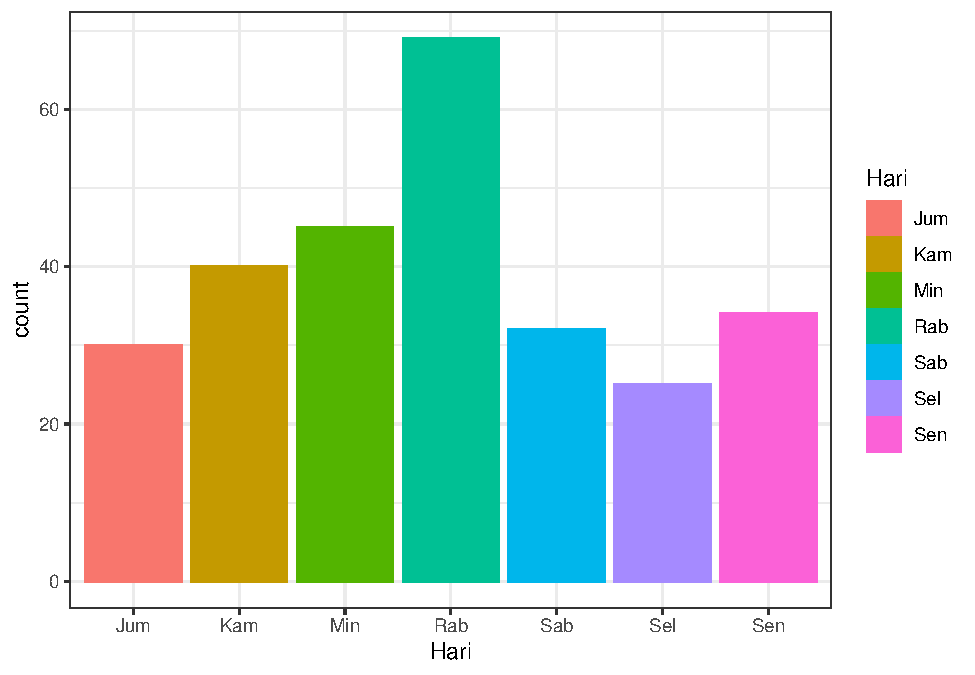
\includegraphics{dr_files/figure-latex/unnamed-chunk-34-1.pdf}

penjelasan:

\begin{itemize}
\tightlist
\item
  \texttt{ggplot(x,\ aes(Hari))} adalah perintah untuk membuat sebuah objek \texttt{ggplot} dari variabel \texttt{Hari} pada data \texttt{x}
\item
  \texttt{geom\_bar(aes(weight=Pasien,\ fill=Hari,\ colour=Hari))}

  \begin{itemize}
  \tightlist
  \item
    \texttt{geom\_bar()} adalah perintah untuk membuat grafik batang menggunakan \texttt{ggplot}
  \item
    \texttt{weight} adalah banyak datanya (dalam kasus yang kita kerjakan: banyaknya Pasien setiap hari)
  \item
    \texttt{fill} bertujuan untuk memberi warna batang (harus sama dengan \texttt{aes(Hari)} pada \texttt{ggplot} agar setiap batang memiliki warna yang berbeda)
  \item
    \texttt{colour} bertujuan untuk memberi warna garis (harus sama dengan \texttt{aes(Hari)} pada \texttt{ggplot} agar setiap batang memiliki warna yang berbeda)
  \end{itemize}
\item
  \texttt{theme\_bw()} bertujuan untuk menentukan tema \texttt{black\ and\ white} pada grafik
\end{itemize}

\hypertarget{grafik-histogram}{%
\section{Grafik Histogram}\label{grafik-histogram}}

Histogram merupakan grafik batang yang dapat menunjukkan seberapa sering suatu nilai yang berbeda terjadi. Histogram lebih sering digunakan untuk melihat distribusi dari suatu data. Berbeda dengan grafik batang, kita perlu menggunakan data numerik dalam membuat sebuah histogram. Berikut adalah data acak yang dibangkitkan dengan perintah \texttt{rnorm}:

\begin{Shaded}
\begin{Highlighting}[]
\NormalTok{data <-}\StringTok{ }\KeywordTok{data.frame}\NormalTok{(}\DataTypeTok{x =} \KeywordTok{rnorm}\NormalTok{(}\DecValTok{100}\NormalTok{,}\DecValTok{5}\NormalTok{,}\DecValTok{2}\NormalTok{))}
\end{Highlighting}
\end{Shaded}

Kita dapat menggunakan perintah \texttt{hist} yang telah tersedia saat melakukan instalasi \texttt{R}.

\begin{Shaded}
\begin{Highlighting}[]
\KeywordTok{hist}\NormalTok{(data}\OperatorTok{$}\NormalTok{x)}
\end{Highlighting}
\end{Shaded}

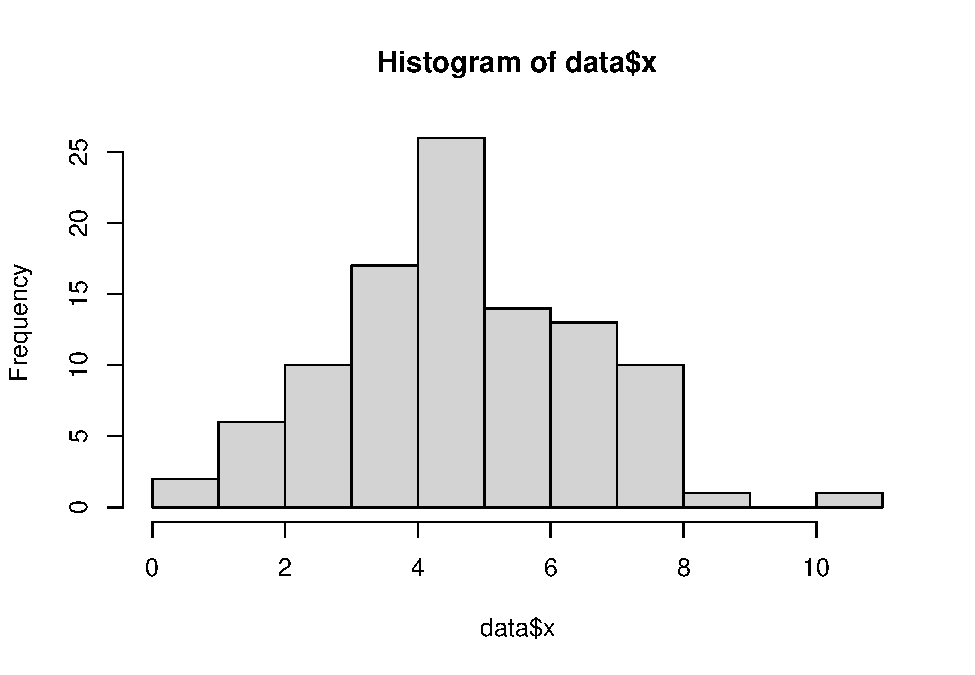
\includegraphics{dr_files/figure-latex/unnamed-chunk-36-1.pdf}

Selanjutnya kita akan menggunakan perintah yang tersedia pada paket \texttt{ggplot2}.

\begin{Shaded}
\begin{Highlighting}[]
\NormalTok{p <-}\StringTok{ }\KeywordTok{ggplot}\NormalTok{(data, }\KeywordTok{aes}\NormalTok{(x)) }\OperatorTok{+}\StringTok{ }
\StringTok{  }\KeywordTok{geom_histogram}\NormalTok{(}\DataTypeTok{binwidth =} \DecValTok{1}\NormalTok{, }
                 \DataTypeTok{color =} \StringTok{"white"}\NormalTok{, }
                 \DataTypeTok{fill=} \StringTok{"darkred"}\NormalTok{) }\OperatorTok{+}
\StringTok{  }\KeywordTok{theme_bw}\NormalTok{()}
\NormalTok{p}
\end{Highlighting}
\end{Shaded}

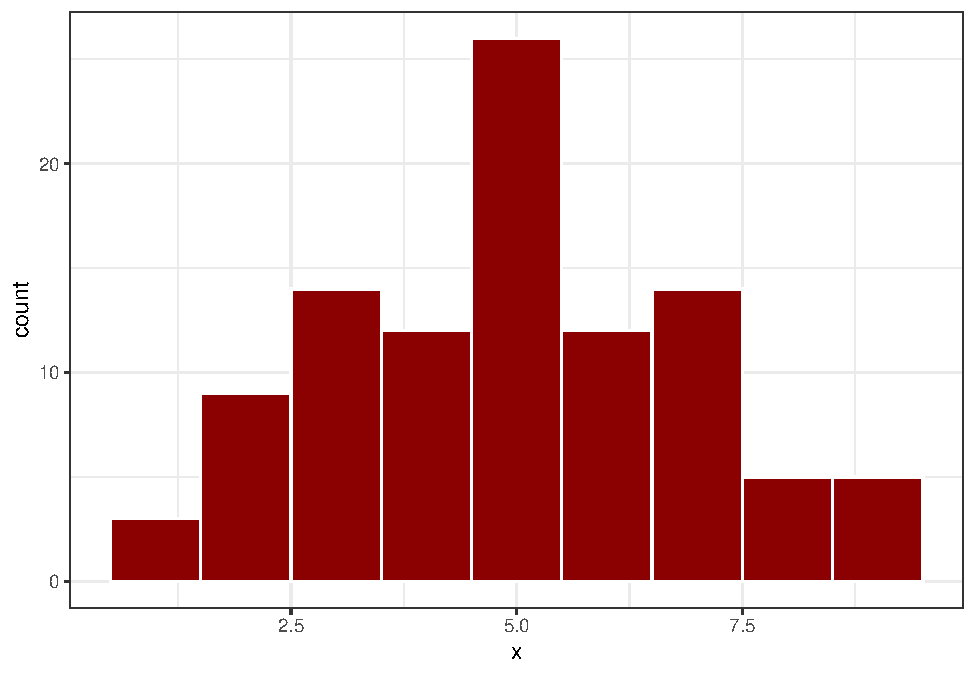
\includegraphics{dr_files/figure-latex/unnamed-chunk-37-1.pdf}

penjelasan:
* \texttt{ggplot(data,\ aes(x))} adalah perintah untuk membuat sebuah objek \texttt{ggplot} dari objek \texttt{x} pada data \texttt{data}
* \texttt{geom\_histogram(binwidth\ =\ 1,\ color\ =\ "white",\ fill=\ "darkred")}
- \texttt{geom\_histogram()} adalah perintah untuk membuat histogram menggunakan \texttt{ggplot}
- \texttt{bandwidth} adalah lebar dari masing-masing batang
- \texttt{fill} bertujuan untuk memberi warna batang (dalam kasus ini kita akan berikan warna yang sama untuk semua batang)
- \texttt{colour} bertujuan untuk memberi warna garis (dalam kasus ini kita akan berikan warna yang sama untuk semua garis)
* \texttt{theme\_bw()} bertujuan untuk menentukan tema \texttt{black\ and\ white} pada plot

Selanjutnya bandingkan dengan histogram yang memiliki \texttt{bandwith} berbeda.

\begin{Shaded}
\begin{Highlighting}[]
\NormalTok{p <-}\StringTok{ }\KeywordTok{ggplot}\NormalTok{(data, }\KeywordTok{aes}\NormalTok{(x)) }\OperatorTok{+}\StringTok{ }
\StringTok{  }\KeywordTok{geom_histogram}\NormalTok{(}\DataTypeTok{binwidth =} \DecValTok{3}\NormalTok{, }
                 \DataTypeTok{color =} \StringTok{"white"}\NormalTok{, }
                 \DataTypeTok{fill=} \StringTok{"darkred"}\NormalTok{) }\OperatorTok{+}
\StringTok{  }\KeywordTok{theme_bw}\NormalTok{()}
\NormalTok{p}
\end{Highlighting}
\end{Shaded}

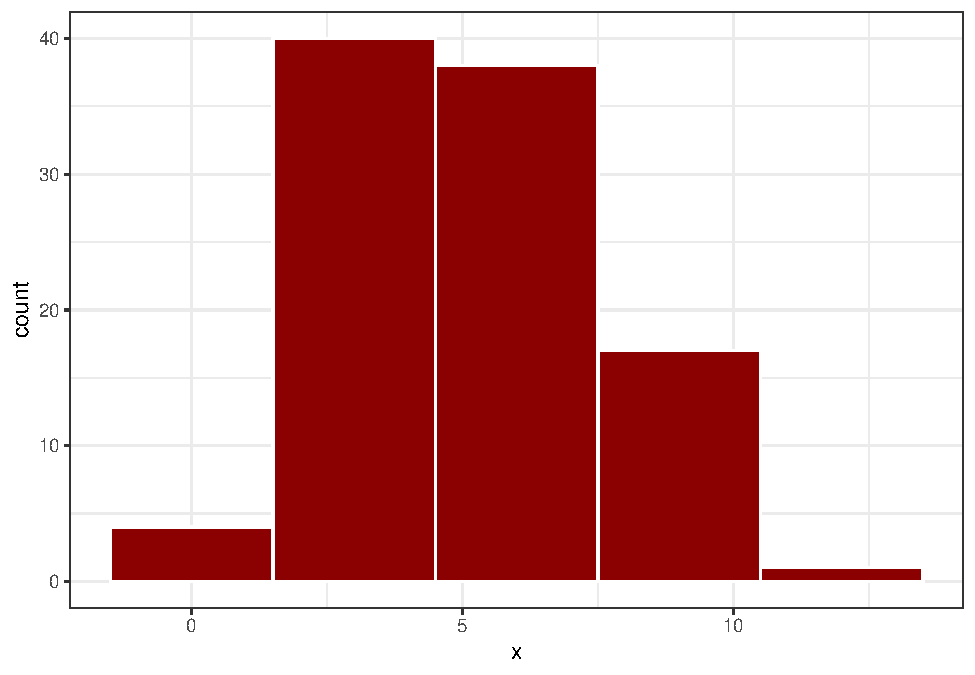
\includegraphics{dr_files/figure-latex/unnamed-chunk-38-1.pdf}

\hypertarget{pie-plot}{%
\section{Pie Plot}\label{pie-plot}}

\begin{Shaded}
\begin{Highlighting}[]
\NormalTok{jumlah <-}\StringTok{ }\KeywordTok{c}\NormalTok{(}\DecValTok{23}\NormalTok{, }\DecValTok{57}\NormalTok{, }\DecValTok{20}\NormalTok{)}
\NormalTok{label <-}\StringTok{ }\KeywordTok{c}\NormalTok{(}\StringTok{"Setuju"}\NormalTok{, }\StringTok{"Tidak setuju"}\NormalTok{, }\StringTok{"Tidak tahu"}\NormalTok{)}
\NormalTok{x <-}\StringTok{ }\KeywordTok{data.frame}\NormalTok{(label, jumlah)}
\end{Highlighting}
\end{Shaded}

Menggunakan perintah \texttt{pie}

\begin{Shaded}
\begin{Highlighting}[]
\KeywordTok{pie}\NormalTok{(x}\OperatorTok{$}\NormalTok{jumlah, }\DataTypeTok{labels =}\NormalTok{ x}\OperatorTok{$}\NormalTok{label)}
\end{Highlighting}
\end{Shaded}

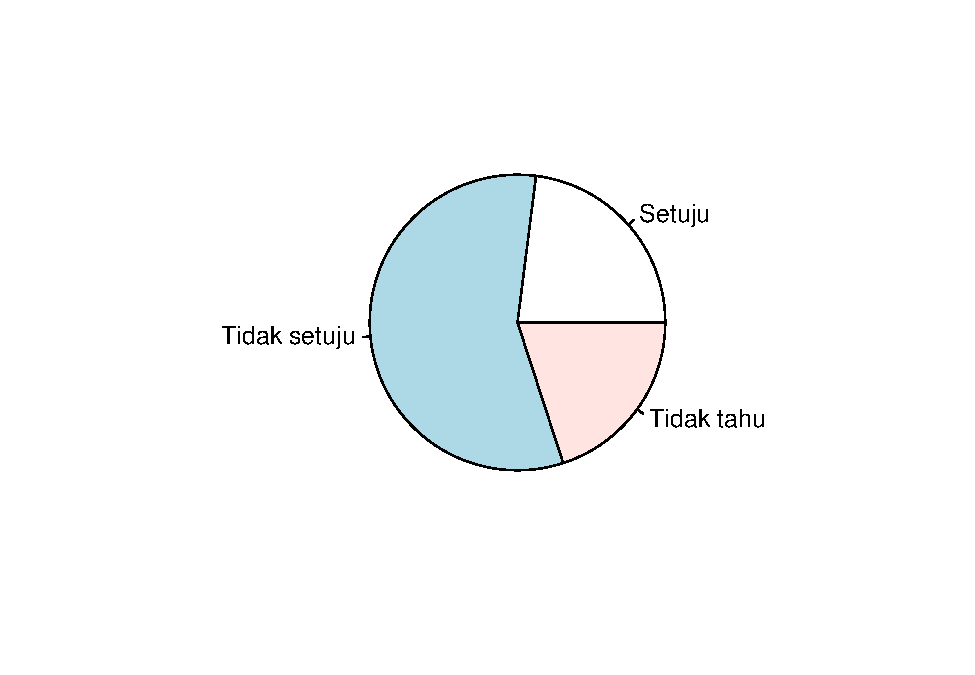
\includegraphics{dr_files/figure-latex/unnamed-chunk-40-1.pdf}

Menggunakan paket \texttt{ggplot2}

\begin{Shaded}
\begin{Highlighting}[]
\NormalTok{p <-}\StringTok{ }\KeywordTok{ggplot}\NormalTok{(x, }\KeywordTok{aes}\NormalTok{(}\DataTypeTok{x=}\StringTok{""}\NormalTok{, }\DataTypeTok{y=}\NormalTok{jumlah, }\DataTypeTok{fill=}\NormalTok{label)) }\OperatorTok{+}
\StringTok{  }\KeywordTok{geom_bar}\NormalTok{(}\DataTypeTok{width =} \DecValTok{1}\NormalTok{, }\DataTypeTok{stat =} \StringTok{"identity"}\NormalTok{)}
\NormalTok{p }\OperatorTok{+}\StringTok{ }\KeywordTok{coord_polar}\NormalTok{(}\StringTok{"y"}\NormalTok{, }\DataTypeTok{start =} \DecValTok{0}\NormalTok{)}
\end{Highlighting}
\end{Shaded}

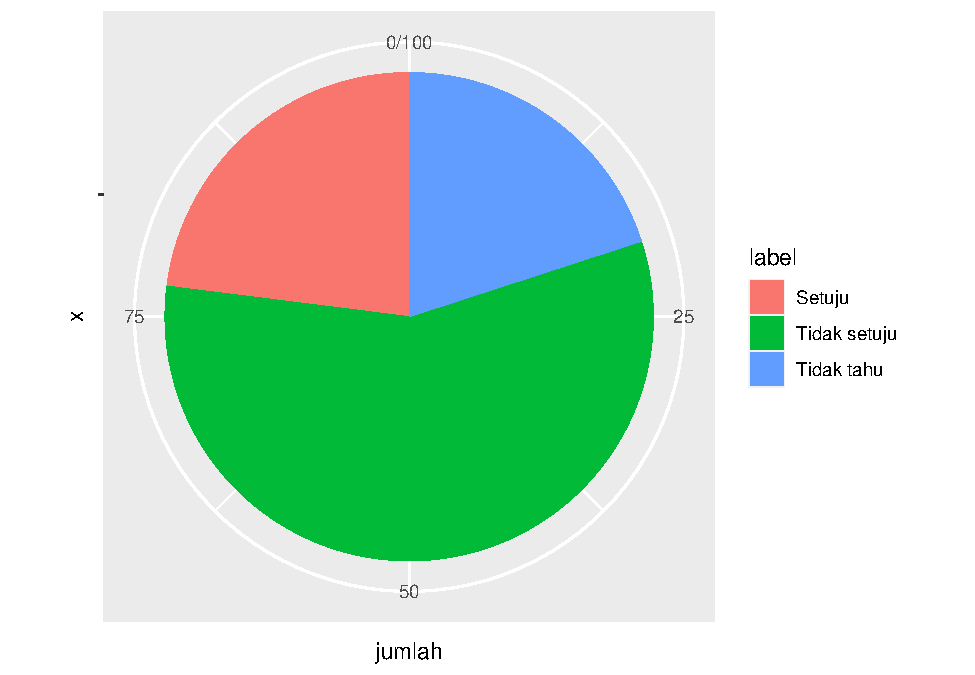
\includegraphics{dr_files/figure-latex/unnamed-chunk-41-1.pdf}

penjelasan:

\hypertarget{box-plot}{%
\section{Box Plot}\label{box-plot}}

\begin{Shaded}
\begin{Highlighting}[]
\NormalTok{x <-}\StringTok{ }\KeywordTok{rnorm}\NormalTok{(}\DecValTok{250}\NormalTok{, }\DecValTok{9}\NormalTok{, }\DecValTok{3}\NormalTok{)}
\NormalTok{y <-}\StringTok{ }\KeywordTok{rnorm}\NormalTok{(}\DecValTok{250}\NormalTok{, }\DecValTok{4}\NormalTok{, }\DecValTok{1}\NormalTok{)}
\NormalTok{z <-}\StringTok{ }\KeywordTok{rnorm}\NormalTok{(}\DecValTok{250}\NormalTok{, }\DecValTok{11}\NormalTok{, }\DecValTok{6}\NormalTok{)}
\end{Highlighting}
\end{Shaded}

Menggunakan perintah \texttt{boxplot}

\begin{Shaded}
\begin{Highlighting}[]
\KeywordTok{boxplot}\NormalTok{(x, y, z,}
        \DataTypeTok{names =} \KeywordTok{c}\NormalTok{(}\StringTok{"x"}\NormalTok{, }\StringTok{"y"}\NormalTok{, }\StringTok{"z"}\NormalTok{))}
\end{Highlighting}
\end{Shaded}

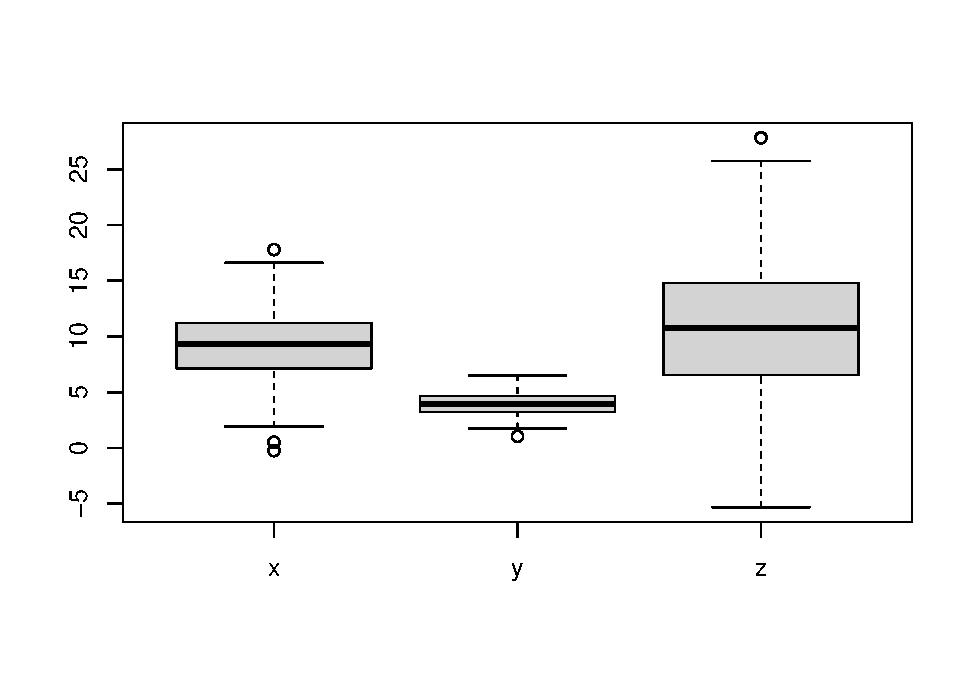
\includegraphics{dr_files/figure-latex/unnamed-chunk-43-1.pdf}

Menggunakan paket \texttt{ggplot2}

\begin{Shaded}
\begin{Highlighting}[]
\NormalTok{data <-}\StringTok{ }\KeywordTok{data.frame}\NormalTok{(}\DataTypeTok{label =} \KeywordTok{c}\NormalTok{(}\KeywordTok{rep}\NormalTok{(}\KeywordTok{c}\NormalTok{(}\StringTok{"x"}\NormalTok{,}\StringTok{"y"}\NormalTok{,}\StringTok{"z"}\NormalTok{),}
                                 \DataTypeTok{each=}\DecValTok{250}\NormalTok{)),}
                   \DataTypeTok{value =} \KeywordTok{c}\NormalTok{(x, y, z))}
\KeywordTok{head}\NormalTok{(data)}
\end{Highlighting}
\end{Shaded}

\begin{verbatim}
##   label     value
## 1     x 11.330038
## 2     x 11.046894
## 3     x  4.841782
## 4     x  9.511102
## 5     x 10.279852
## 6     x 14.465684
\end{verbatim}

\begin{Shaded}
\begin{Highlighting}[]
\NormalTok{p <-}\StringTok{ }\KeywordTok{ggplot}\NormalTok{(data, }\KeywordTok{aes}\NormalTok{(}\DataTypeTok{x=}\NormalTok{label, }\DataTypeTok{y=}\NormalTok{value)) }\OperatorTok{+}
\StringTok{  }\KeywordTok{geom_boxplot}\NormalTok{(}\DataTypeTok{outlier.colour =} \StringTok{"red"}\NormalTok{) }\OperatorTok{+}
\StringTok{  }\KeywordTok{theme_bw}\NormalTok{()}
\NormalTok{p}
\end{Highlighting}
\end{Shaded}

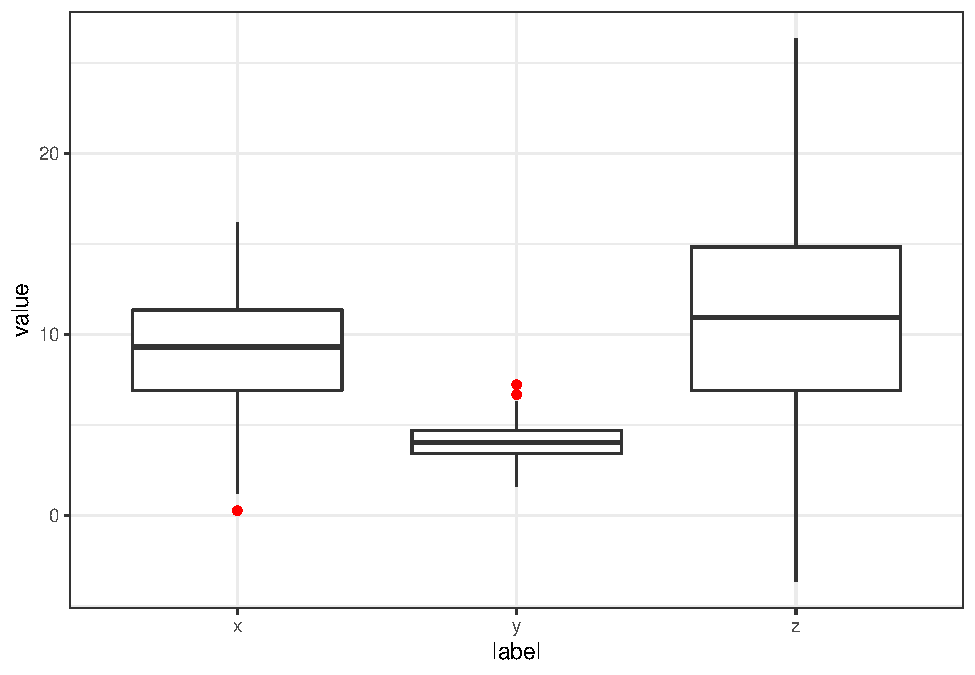
\includegraphics{dr_files/figure-latex/unnamed-chunk-44-1.pdf}

\hypertarget{line-plot}{%
\section{Line Plot}\label{line-plot}}

\begin{Shaded}
\begin{Highlighting}[]
\NormalTok{x <-}\StringTok{ }\KeywordTok{c}\NormalTok{(}\DecValTok{23}\NormalTok{, }\DecValTok{57}\NormalTok{, }\DecValTok{20}\NormalTok{)}
\KeywordTok{names}\NormalTok{(x) <-}\StringTok{ }\KeywordTok{c}\NormalTok{(}\StringTok{"Setuju"}\NormalTok{, }\StringTok{"Tidak setuju"}\NormalTok{, }\StringTok{"Tidak tahu"}\NormalTok{)}
\end{Highlighting}
\end{Shaded}

Menggunakan perintah \texttt{pie}

\begin{Shaded}
\begin{Highlighting}[]
\KeywordTok{plot}\NormalTok{(x, }\DataTypeTok{type =} \StringTok{"o"}\NormalTok{)}
\end{Highlighting}
\end{Shaded}

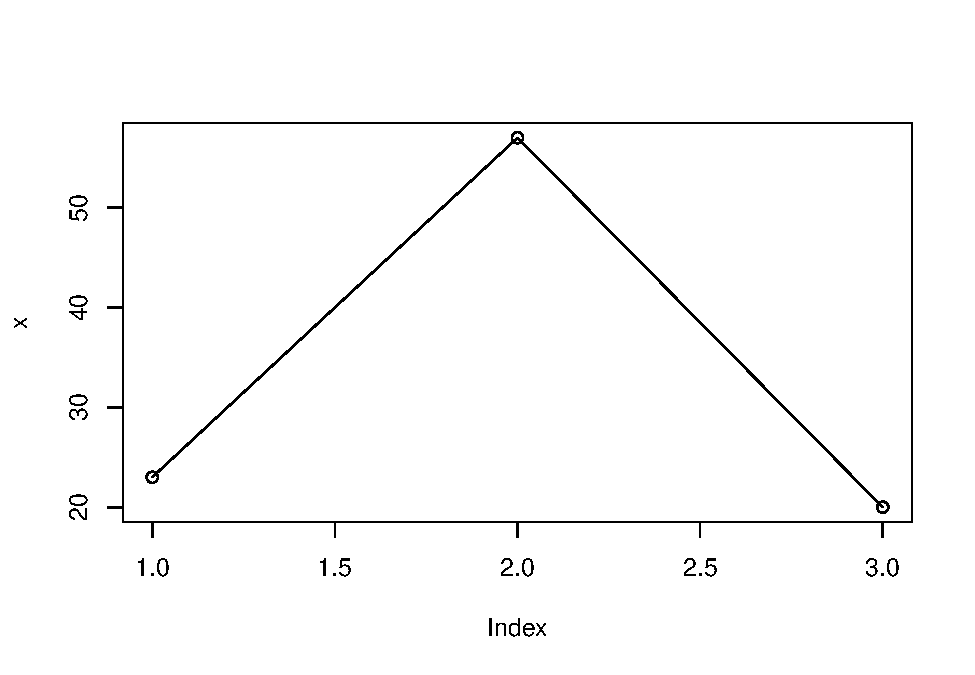
\includegraphics{dr_files/figure-latex/unnamed-chunk-46-1.pdf}

Menggunakan paket \texttt{ggplot2}

\hypertarget{scatter-plot}{%
\section{Scatter Plot}\label{scatter-plot}}

\begin{Shaded}
\begin{Highlighting}[]
\NormalTok{x <-}\StringTok{ }\KeywordTok{c}\NormalTok{(}\DecValTok{23}\NormalTok{, }\DecValTok{57}\NormalTok{, }\DecValTok{20}\NormalTok{)}
\KeywordTok{names}\NormalTok{(x) <-}\StringTok{ }\KeywordTok{c}\NormalTok{(}\StringTok{"Setuju"}\NormalTok{, }\StringTok{"Tidak setuju"}\NormalTok{, }\StringTok{"Tidak tahu"}\NormalTok{)}
\end{Highlighting}
\end{Shaded}

Menggunakan perintah \texttt{pie}

\begin{Shaded}
\begin{Highlighting}[]
\KeywordTok{pie}\NormalTok{(x, }\DataTypeTok{labels =} \KeywordTok{names}\NormalTok{(x))}
\end{Highlighting}
\end{Shaded}

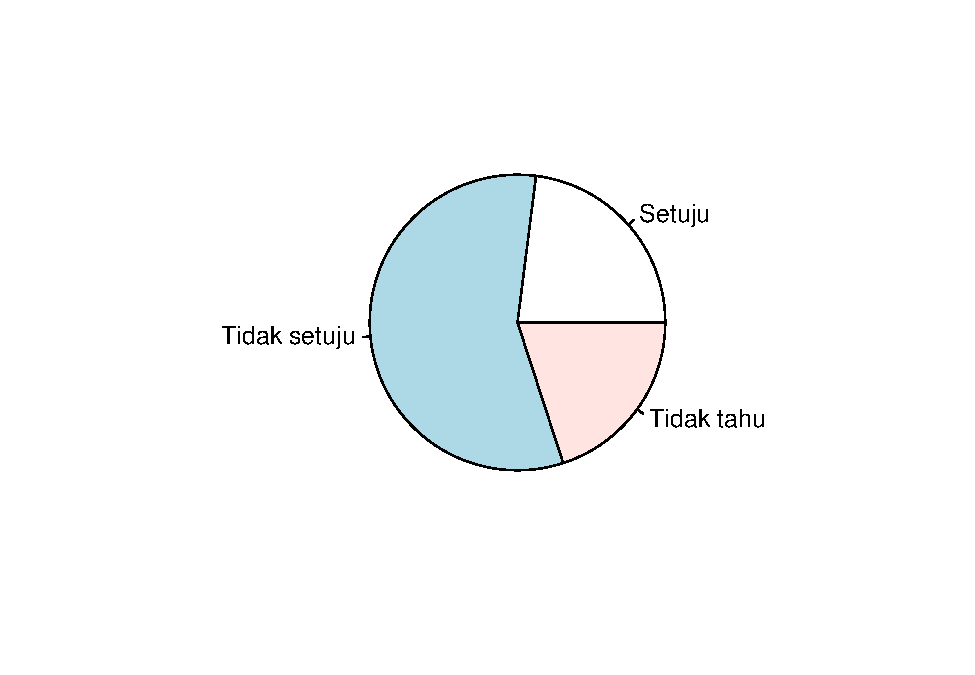
\includegraphics{dr_files/figure-latex/unnamed-chunk-48-1.pdf}

Menggunakan paket \texttt{ggplot2}

\hypertarget{area-plot}{%
\section{Area Plot}\label{area-plot}}

\begin{Shaded}
\begin{Highlighting}[]
\NormalTok{x <-}\StringTok{ }\KeywordTok{c}\NormalTok{(}\DecValTok{23}\NormalTok{, }\DecValTok{57}\NormalTok{, }\DecValTok{20}\NormalTok{)}
\KeywordTok{names}\NormalTok{(x) <-}\StringTok{ }\KeywordTok{c}\NormalTok{(}\StringTok{"Setuju"}\NormalTok{, }\StringTok{"Tidak setuju"}\NormalTok{, }\StringTok{"Tidak tahu"}\NormalTok{)}
\end{Highlighting}
\end{Shaded}

Menggunakan perintah \texttt{pie}

\begin{Shaded}
\begin{Highlighting}[]
\KeywordTok{pie}\NormalTok{(x, }\DataTypeTok{labels =} \KeywordTok{names}\NormalTok{(x))}
\end{Highlighting}
\end{Shaded}

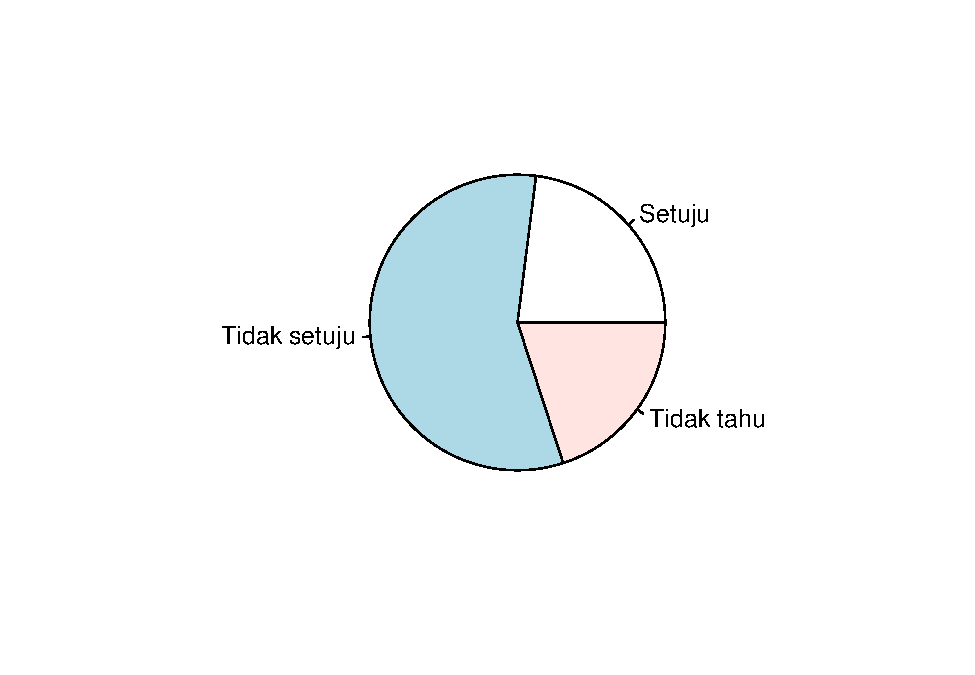
\includegraphics{dr_files/figure-latex/unnamed-chunk-50-1.pdf}

Menggunakan paket \texttt{ggplot2}

  \bibliography{book.bib,packages.bib}

\end{document}
